\chapter{Topics, Domains and Partitions}\label{Chapter:Topics:Domain:Partitions}
In the previous chapter I introduced the basics of DDS and 
walked you through the steps required to write a simple pub/sub 
application. Now it is time to start looking in more depth at DDS 
and we have no better place to start than data management.

\section{Topics Inside Out}
A topic represents the unit for information that can produced 
or consumed by a \ac{DDS} application. Topics are defined by a name, a type, 
and a set of \ac{QoS} policies. 

\subsection{Topic Types}
As \ac{DDS} is independent of the programming language as well as the \ac{OS}
it defines its type system \index{type system} ~\cite{OMG:DDS:XTYPES:10} along with an space and time 
efficient binary encoding for its types. 
Different syntaxes can be used to express \ac{DDS} topic types, such as IDL, XML, and annotated Java. 

In this Tutorial I will be focusing on the subset of \ac{IDL} that can be used 
to define a topic type. A topic type is made by an \ac{IDL}  struct plus a key.  
The struct can contain as many fields as you want and each field  can be a 
primitive type (see Table~\ref{Table:Primitive:Types}),  a template type 
(see Table~\ref{Table:Template:Types}), or a  constructed type 
(see Table~\ref{Table:Contructed:Types}).


\begin{table}
\begin{center}
{\small
\begin{tabular}{|c|c|}
\hline 
{\textbf{Primitive Types}} &  \textbf{ Size (bits) }\\ 
\hline 
\begin{lstlisting}
boolean
\end{lstlisting} & 
\begin{lstlisting}
8
\end{lstlisting} \\ \hline 
\begin{lstlisting}
octet 
\end{lstlisting}  & 
\begin{lstlisting}
8
\end{lstlisting} \\ \hline 
\begin{lstlisting} 
char
\end{lstlisting}   & 
\begin{lstlisting}
8
\end{lstlisting} \\ \hline 
\begin{lstlisting}
wchar
\end{lstlisting}   &
\begin{lstlisting}
16
\end{lstlisting} \\ \hline 
\begin{lstlisting}
short
\end{lstlisting}   &
\begin{lstlisting}
16
\end{lstlisting} \\ \hline 
\begin{lstlisting}
unsigned short
\end{lstlisting}  & 
\begin{lstlisting}
16
\end{lstlisting} \\ \hline 
\begin{lstlisting}
long
\end{lstlisting}  &
\begin{lstlisting}
32
\end{lstlisting} \\ \hline 

\begin{lstlisting}
unsigned long
\end{lstlisting}  &
\begin{lstlisting}
32
\end{lstlisting} \\ \hline 

\begin{lstlisting}
long long
\end{lstlisting}  &
\begin{lstlisting}
64
\end{lstlisting} \\ \hline 

\begin{lstlisting}
unsigned long long
\end{lstlisting}  &
\begin{lstlisting}
64
\end{lstlisting} \\ \hline 
\begin{lstlisting}
float
\end{lstlisting}  &
\begin{lstlisting}
32
\end{lstlisting} \\ \hline 
\begin{lstlisting}
double
\end{lstlisting}  &
\begin{lstlisting}
64
\end{lstlisting} \\ \hline 
\end{tabular}
}
\label{Table:Primitive:Types} 
\end{center}
\end{table}

As shown in Table~\ref{Table:Primitive:Types}, primitive types are essentially 
what you'd expect, with just one exception -- the int type is not there!  
This should not worry you since the IDL integral types short, long and long long 
are equivalent to the C99 int16\_t, int32\_t and int64\_t thus you have all you need. 
%%%
\begin{table}
\begin{center}
{\small
\begin{tabular}{|c|l|}

\hline
	\textbf{Template Type} &  \textbf{Example}  \\
\hline
\begin{lstlisting}
string<length = UNBOUNDED$>
\end{lstlisting}    & % ROW 1
    
\begin{lstlisting}
string s1;
string<32> s2;
\end{lstlisting} \\ 

\hline 
\begin{lstlisting}
wstring<length = UNBOUNDED>
\end{lstlisting}    & % ROW 2
\begin{lstlisting}
wstring ws1;
wstring<64> ws2; 
\end{lstlisting} \\

\hline 
\begin{lstlisting}
sequence<T,length = UNBOUNDED>
\end{lstlisting}  & % ROW 3
\begin{lstlisting} 
sequence<octet> oseq;
sequence<octet, 1024> oseq1k;
sequence<MyType> mtseq;																			
sequence<MyType, $10>$ mtseq10;
\end{lstlisting} \\
\hline 
\begin{lstlisting}
fixed<digits,scale>
\end{lstlisting} &  % ROW 4
\begin{lstlisting}
fixed<5,2> fp; //d1d2d3.d4d5
\end{lstlisting} \\
\hline 
\end{tabular}
}
\caption{IDL Template Types}
\label{Table:Template:Types} 
\end{center}
\end{table}
%%%
Table~\ref{Table:Template:Types} shows IDL templates types. The \texttt{string} 
and \texttt{wstring} can be parametrized only with respect to their maximum 
length; the sequence type with respect to its length and  contained type; 
the fixed type with respect to the total number of digits and the scale. 
The sequence type abstracts homogeneous random access container, pretty 
much like the \texttt{std::vector} in C++ or \texttt{java.util.Vector} in Java. Finally, 
it is important to point out that when the maximum length is not provided 
the type is assumed as having an unbounded length, meaning that the
middleware will allocate as much memory as necessary to store the values 
the application provides.
%%%
\begin{table}
\begin{center}
{\small
\begin{tabular}{|c|l|}

\hline
	\textbf{Constructed Type} & \textbf{Example}  \\
\hline
%% Col 1
\begin{lstlisting}
enum
\end{lstlisting}     &  % ROW 1
\begin{lstlisting}
enum Dimension {1D, 2D, 3D, 4D}; 
\end{lstlisting} \\    
\hline 
\begin{lstlisting}
struct
\end{lstlisting}      & % ROW 2  
\begin{lstlisting}
struct Coord1D { long x;};
struct Coord2D { long x; long y; };
struct Coord3D { long x; long y; long z; }; 
struct Coord4D { long x; long y; long z,
                 unsigned long long t;};
\end{lstlisting} \\ 
\hline 
\begin{lstlisting}
union
\end{lstlisting}      & % ROW 3
\begin{lstlisting}
union Coord switch (Dimension) {  
   case 1D: Coord1D c1d;
   case 2D: Coord2D c2d;
   case 3D: Coord3D c3d;
   case 4D: Coord4D c4d;
};
\end{lstlisting} \\

\hline 
\end{tabular}
}
\caption{IDL Template Types}
\label{Table:Contructed:Types} 
\end{center}
\end{table}
%%%
Table~\ref{Table:Contructed:Types} shows that \ac{DDS} supports three different 
kinds of \ac{IDL} constructed types, \texttt{enum}, \texttt{struct}, and \texttt{union}. 
Putting it all together, you should now realize that a Topic type is a struct that 
can contain as fields nested structures, unions ,enumerations, template types as 
well as primitive types. In addition to this, you can define  multi-dimensional 
arrays of any DDS-supported or user-defined type. 

This is all nice, but you might wonder how this it ties-in with programming 
languages such as C++, Java, C\#. The answer is not really surprising, essentially 
there is a language-specific mapping from the IDL-types described above to mainstream
programming languages.

\subsection{Topic Keys, Instances and Samples}\label{Section:Keys:Instance:Samples}
Each Topic comes with an associated key-set. This key-set might be empty or it 
can include an arbitrary number of attributes defined by the Topic Type. There are 
no limitations on the number, kind, or level of nesting, of attributes used to establish the key.

\lstinputlisting[
		frame=b,
		label={Listing:IDL:KeyedAndKeyLessTopics},
		caption={Keyed and Keyless Topics.}]
		{./listing/idl/KeyNoKeyTempSensor.idl}

If we get back to our running example, the temperature control and monitoring 
system, we could define a keyless variant of the \texttt{TempSensorType}  defined in 
Chapter~\ref{Chapter:Foundations}. Listing~\ref{Listing:IDL:KeyedAndKeyLessTopics} 
shows our old good \texttt{TempSensorType} 
with the id attribute defined as its key,  along with the 
\texttt{KeylessTempSensorType} showing-off an empty key-set as 
defined in its \#pragma keylist directive.

If we create two topics associated with the types declared in 
Listing~\ref{Listing:IDL:KeyedAndKeyLessTopics} what would be the exact 
difference between them? 
\iftoggle{cpp}{
\lstinputlisting[
		frame=tb,
		label={Listing:DDS:CreateKeyedAndKeyLessTopics}]
		{./listing/cxx/KeyNoKeyTopicCreation.cpp}
}

The main difference between these two topics is their number of instances. 
Keyless topics have only once instance, thus can be thought as singletons. 
Keyed topics have once instance per key-value.   Making a parallel with classes 
in object oriented programming languages, you can think of a Topic as defining 
a class whose instances are created for each unique value of the topic keys. 
Thus if the topic has no keys you get a singleton. 

Topic instances are runtime entities for which DDS keeps track of 
whether (1) there are any live writers, (2) the instance has appeared 
in the system for the first time, and (3) the instance has been 
disposed--meaning explicitly removed from the system. 
Topic instances impact the organization of data on the reader side as 
well as the memory usage. Furthermore, as we will see later on in the series, 
there are some QoS that apply at an instance-level.

Let me now illustrate what happens when you write a keyless topic 
versus a keyed topic. If we write a sample for the  \texttt{KLSensorTopic} 
this is going to modify the value for  exactly the same instance,
the singleton, regardless of the content of the sample.
 On the other, each sample you write for the \texttt{TempSensorTopic} 
 will modify the value of a specific topic instance, depending on 
 the value of the key attributes, the id in our example. 

Thus, the code below is writing two samples for the same instance, as shown in 
Figure~\ref{Figure:DDS:DRCache:NoKey:Topic}.
%%%
\iftoggle{cpp}{
\lstinputlisting[
		frame=tb,
		label={Listing:DDS:CreateKeyedAndKeyLessTopics}]
		{./listing/cxx/WriteInstanceExample.cpp}
} \\
%%%

These two samples will be posted in the same reader queue; the queue 
associated with the singleton instance, as shown in Figure~\ref{Figure:DDS:DRCache:NoKey:Topic}.
%%%
\begin{figure}[ht]
	\centering
	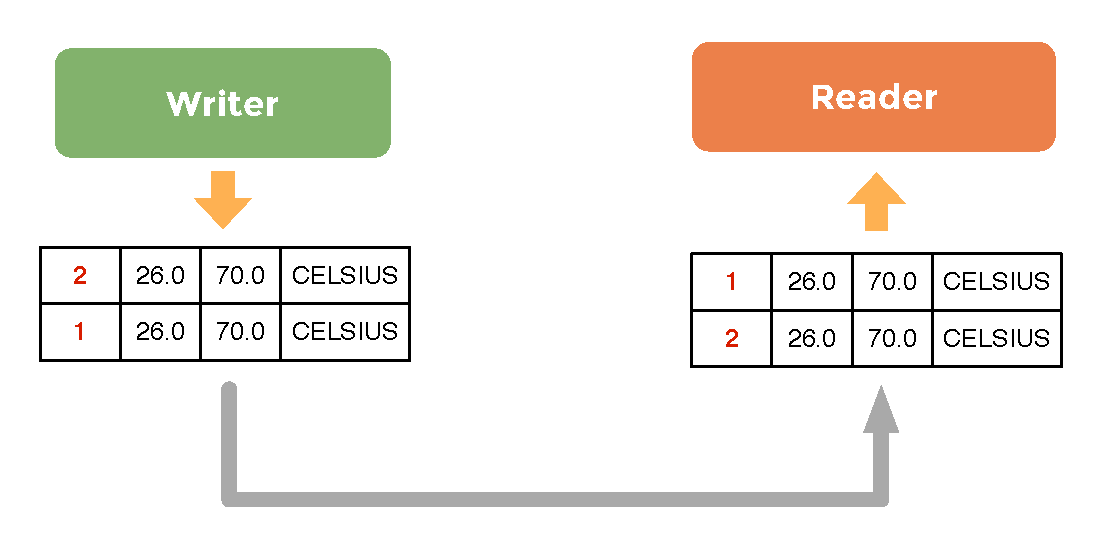
\includegraphics[scale=0.5]{figs/keyless-topic.eps}
	\caption{Data Reader queues for a keyless Topics.}
	\label{Figure:DDS:DRCache:NoKey:Topic}
\end{figure}
%%%
If we write the same samples for the \texttt{TempSensorTopic}, 
the end-result is quite different. The two samples written in the 
code fragment below have two different id values, respectively 1 and 2, 
as a result they are referring to two different instances. 
%%%
\iftoggle{cpp}{
\lstinputlisting[
		frame=tb,
		label={Listing:DDS:CreateKeyedAndKeyLessTopics}]
		{./listing/cxx/WriteKeyedInstanceExample.cpp}
}
%%%
In this case the reader will see these two samples posted into two different queues, 
as represented in Figure~\ref{Figure:DDS:DRCache:Keyed:Topic}, one queue for each instance. 
%%%
\begin{figure}[ht]
	\centering
	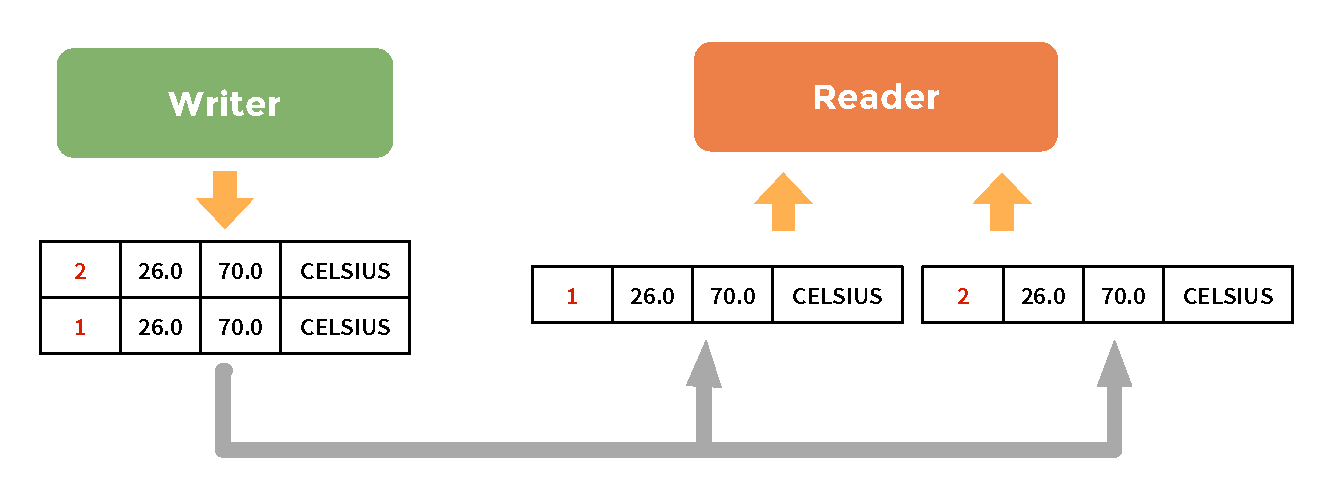
\includegraphics[scale=0.5]{figs/keyed-topic.eps}
	\caption{Data Reader queues for a keyed Topics.}
	\label{Figure:DDS:DRCache:Keyed:Topic}
\end{figure}
%%%
In summary, you should think of Topics as classes in an object oriented 
language and understand that each unique key-value identifies an instance. 
The life-cycle of topic instances is managed by DDS and to each topic instance 
are associated memory resources, you can think of it as a queue on the reader side.  
Keys identify specific data streams within a Topic. Thus, in our running example, 
each id value will identify a specific temperature sensor. 
Differently from many other \ac{Pub/Sub} technologies, \ac{DDS} allows you to 
use keys to automatic demultiplex different streams of data. 
Furthermore, since each temperature sensor will be representing an instance of 
the \texttt{TempSensorTopic} you'll be able to track the lifecycle of the sensor 
by tracking the lifecycle of its associated instance. 
You can detect when a new sensor is added into the system, just because 
it will introduce a new instance, you can detect when a sensor has failed, 
thanks to the fact that DDS can inform you when there are no more writers for a 
specific instance. You can even detect when a sensor has crashed and then recovered 
thanks to some information about the state transition that are provided by \ac{DDS}. 

Finally, before setting to rest \ac{DDS} instances, I want to underline 
that \ac{DDS} subscriptions concerns Topics. As a result when subscribing to a topic, 
you'll receive all the instances produced for that topic.  In some cases this is 
not desirable and some scoping actions are necessary. Let's see then what DDS has to offer.

\section{Scoping Information}\label{Section:Scoping:Information}
\subsection{Domain}
DDS provides two mechanism for scoping information, domains and partitions.
A domain establishes a virtual network linking all the \ac{DDS} applications 
that have joined it. 
No communication can ever happen across domains unless explicitly mediated 
by the user application. 
\subsection{Partition}
Domains can be further organized into partitions, where each partition represent 
a logical grouping of topics. DDS Partitions are described by names such 
as "SensorDataPartition", "CommandPartition", "LogDataPartition", etc., 
and have to be explicitly joined in order to publish data in it or subscribe 
to the topics it contains. The mechanism provided by \ac{DDS} for joining a 
partition is very flexible as a publisher or a subscriber can join by providing 
its full name, such as "SensorDataPartition" or it can join all the partitions 
that match a regular expression, such as "Sens*", or "*Data*". 
Supported regular expressions are the same as those accepted by the POSIX 
\texttt{fnmatch} \cite{POSIX:fmatch} function. 

To recap, partitions provide a way of scoping information. 
You can use this scoping mechanism to organize topics into different coherent sets. 
You can equally use partitions to segregate topic instances.  
Instance segregation can be necessary for optimizing performance or minimizing 
footprint for those applications that are characterized by a very large number 
of instances, such as large telemetry systems, or financial trading applications.
If we take as an example our temperature monitoring and control system, 
then we can devise with a very natural partitioning of data that mimics the 
physical placement of the various temperature sensors.  To do this, we can use 
a partition naming scheme made of the building number, the floor level and the 
room number in which the sensor is installed:
\begin{center}
  \texttt{"building-<number>:floor-<level>:room-<number>"}
\end{center}
Using this naming scheme, as shown in Figure~\ref{Figure:DDS:Partitions}, 
all the topics produced 
in room 51 on the 15th floor on building 1 would belong to the partition 
\texttt{"building-1:floor-15:room-51"}. Likewise, the partition expression 
\texttt{"building-1:floor-1:room-*"} matches all the partitions for the rooms at 
the first floor in building.
%%%
\begin{figure}[t]
	\centering
	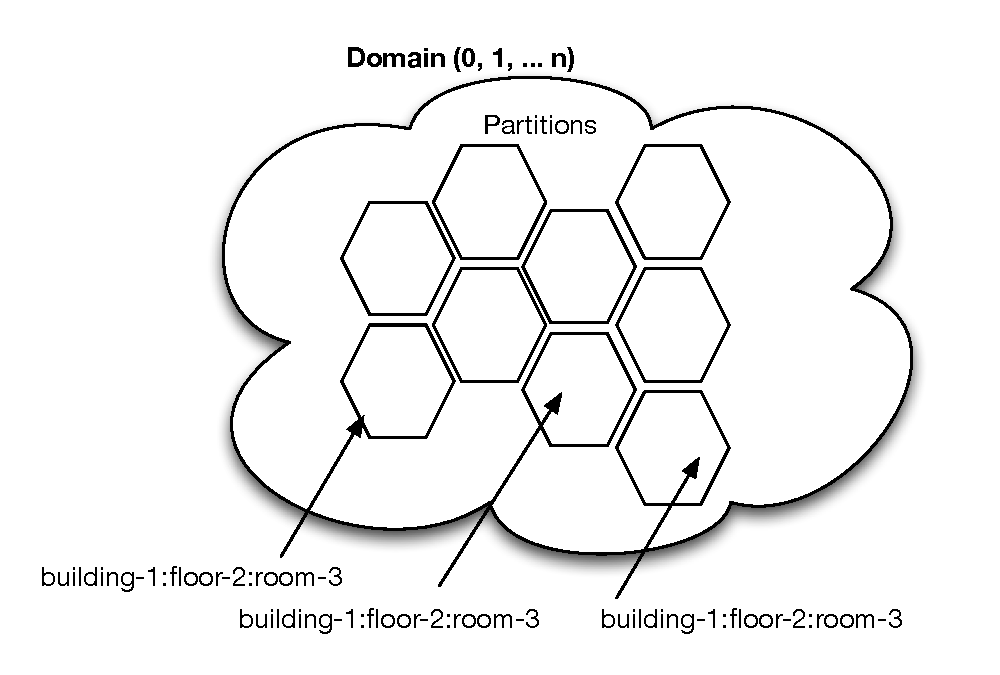
\includegraphics[scale=0.7]{figs/domain-partitions.eps}
	\caption{Domain and partitions in DDS.}
	\label{Figure:DDS:Partitions}
\end{figure}
%%%

In a nutshell,  you can use partitions to scope information, you can also 
use naming conversions such as those used for our temperature control 
applications to emulate hierarchical organization of data starting from 
flat partitions. Using the same technique you can slice and access data 
across different dimensions or views, depending on the need of your application.
%%%
%%%
%%%
\section{Content Filtering}~\label{Section:Content:Filtering}
Domains and Partitions are useful mechanisms for structurally organizing data, 
but what if you need to control the data received based on its content? 
Content Filtering allows you to create topics that constrain the 
values their instances might take. When subscribing to a content-filtered 
topic an application will only receive, among all published values, 
only those that match the topic filter.  The filter expression can 
operate on the full topic content, as opposed to being able to operate 
only on headers as it happens in many other pub/sub technologies, 
such as JMS. The filter expression is structurally similar to a SQL WHERE clause.
The operators supported by are listed in Table~\ref{Table:DDS:Filter:Expression}.
%%%
%%%

\begin{table}
\begin{center}
{\footnotesize\ttfamily
\begin{tabular}{|c|l|} \hline
\textbf{Constructed Type} 	&  	\textbf{Example}  			\\ \hline
              =           	&  	equal  						\\ \hline
              <>          	&  	not equal					\\ \hline
              >           	&  	greater than  				\\ \hline
              <				& 	less than					\\ \hline
              >=				& 	greater than or equal 		\\ \hline
              <=				&	less than or equal			\\ \hline
              BETWEEN		&   between and inclusive range	\\ \hline
              LIKE			&	matches a string pattern		\\ \hline               
\end{tabular}}
\end{center}
\label{Table:DDS:Filter:Expression}
\caption{Legal operators for  DDS Filters and Query Conditions}
\end{table}
%%%
%%%
%%%
Content-Filtered topics are very useful from several different perspectives. 
First of all they limit the amount of memory used by \ac{DDS} to the 
instances and samples that match the filter.  Furthermore, filtering can be 
used to simplify your application by delegating to DDS the logic that checks 
certain data properties. For instance, if we consider our temperature control 
application we might be interested in being notified only then the temperature 
or the humidity are outside a given range. 
Thus assuming we wanted to maintain the temperature between $20.5\,^{\circ}\mathrm{C}$ and 
$21.5\,^{\circ}\mathrm{C}$ and the humidity between $30\%$ and $50\%$, 
we could create a Content-Filtered topic that would alert the application when the 
sensor is producing value outside our desired set point.  This can be done by using the 
filter expression below:
%%%

\begin{lstlisting}[frame=tb]
       ((temp NOT BETWEEN (20.5 AND 21.5)) 
          OR 
       (hum NOT BETWEEN (30 AND 50)))
\end{lstlisting}
%%%
Listing~\ref{Listing:DDS:ContentFiltered:Topic} shows the code that creates a 
content-filtered topic for the TempSensor topic  with the expression above. 
Notice that the content-filtered topic is created starting from a regular topic. 
Furthermore it is worth noticing that the filter expression  is relying on positional 
arguments $\%0$, $\%2$, etc., whose actual values are passed via a vector of strings. 

%%%
\iftoggle{cpp}{
	\lstinputlisting[
		frame=b,
		label={Listing:DDS:ContentFiltered:Topic},
		caption={Content Filtered Topic.}]
		{./listing/cxx/content-filtered-topic.cpp}
}
%%%


\section{Summary}
In this chapter I have covered the most important aspects of data management in DDS. 
By now you've learned all you needed to know about topics-types and topic instances 
and you've been exposed to the the various mechanism provided by DDS for scoping 
information. In summary, you can organize structurally your information by means 
of domains and partitions. Then you can create special views using content-filtered 
topics and query conditions.
At this point my usual suggestion is that you try to compile and run the examples 
and try to experiment a bit by yourself.

